\documentclass[paper=a4, fontsize=11pt]{scrartcl} 

\usepackage[T1]{fontenc} 
\usepackage[english]{babel}
\usepackage{amsmath,amsfonts,amsthm}

\usepackage{lipsum}

\usepackage{graphicx}
\usepackage{float}
  \floatplacement{figure}{H}
  \floatplacement{table}{H}
  
\usepackage{sectsty} 
\allsectionsfont{\centering \normalfont\scshape} 

\usepackage{fancyhdr} % Custom headers and footers
\pagestyle{fancyplain} % Makes all pages in the document conform to the custom headers and footers
\fancyhead{} % No page header - if you want one, create it in the same way as the footers below
\fancyfoot[L]{} % Empty left footer
\fancyfoot[C]{} % Empty center footer
\fancyfoot[R]{\thepage} % Page numbering for right footer
\renewcommand{\headrulewidth}{0pt} % Remove header underlines
\renewcommand{\footrulewidth}{0pt} % Remove footer underlines
\setlength{\headheight}{13.6pt} % Customize the height of the header

\numberwithin{equation}{section} % Number equations within sections (i.e. 1.1, 1.2, 2.1, 2.2 instead of 1, 2, 3, 4)
\numberwithin{figure}{section} % Number figures within sections (i.e. 1.1, 1.2, 2.1, 2.2 instead of 1, 2, 3, 4)
\numberwithin{table}{section} % Number tables within sections (i.e. 1.1, 1.2, 2.1, 2.2 instead of 1, 2, 3, 4)

\setlength\parindent{0pt} % Removes all indentation from paragraphs - comment this line for an assignment with lots of text

%----------------------------------------------------------------------------------------
%	TITLE SECTION
%----------------------------------------------------------------------------------------

\newcommand{\horrule}[1]{\rule{\linewidth}{#1}} % Create horizontal rule command with 1 argument of height

\title{	
\normalfont \normalsize 
\textsc{Computational Science - ITB} \\ [25pt] % Your university, school and/or department name(s)
\horrule{0.5pt} \\[0.4cm] % Thin top horizontal rule
%\huge  Summary - Euler Method\\ % The assignment title
%\horrule{2pt} \\[0.5cm] % Thick bottom horizontal rule
}

\author{\small{Ridlo W. Wibowo || 20912009}} % Your name

\date{\normalsize\today} % Today's date or a custom date

\begin{document}

\maketitle % Print the title

\large \textbf{Problem 1.}
Buatlah program \textit{Cubic Spline Interpolation},\\
- \textit{Natural}\\ 
- \textit{Clamped}\\

\large \textbf{Problem 2.}
Construct the natural cubic spline for the following data.\\
\begin{table}[ht]
%\caption{Nonlinear Model Results} % title of Table
%\centering  % used for centering table
\begin{tabular}{c c} % centered columns (4 columns)
\hline%\hline                        %inserts double horizontal lines
x & f(x) \\ [0.5ex] % inserts table 
%heading
\hline                  % inserts single horizontal line
0.1 & -0.62049958 \\
0.2 & -0.28398668 \\
0.3 & 0.00660095 \\
0.4 & 0.24842440 \\ [1ex]
\hline %inserts single line
\end{tabular}
%\label{table:nonlin} % is used to refer this table in the text
\end{table}
\begin{table}[ht]
\begin{tabular}{c c}
\hline
x & f(x) \\ [0.5ex]
\hline 
-1 & 0.86199480 \\
-0.5 & 0.95802009 \\
0 & 1.0986123 \\
0.5 & 1.2943767 \\ [1ex]
\hline 
\end{tabular}
\end{table}

\large \textbf{Problem 3.}
The data in Problem 2. were generated using the following functions. Use the cubic splines constructed in Problem 2. for the given value of x to approximate $f(x)$ and $f'(x)$, and calculate the actual error.\\

$f(x) = xcos(x) - 2x^{2} + 3x - 1$; approximate $f(0.25)$ and $f'(0.25)$.\\

$f(x) = ln(e^{x} + 2)$; approximate $f(0.25)$ and $f'(0.25)$.\\

\large \textbf{Problem 4.}
It is suspected that the high amounts of tannin in mature oak leaves inhibit the growth of the winter moth (Operophtera \textit{bromata L., Geometridae}) larvae that extensively damage these trees in certain years. The following table lists the average weight of two samples of larvae at times in the first 28 days after birth. The first sample was reared on young oak leaves, whereas the second sample was reared on mature leaves from the same tree.
\begin{figure}
	\centering
	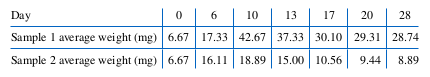
\includegraphics[width=0.8\textwidth]
		{data4.png}
	%\caption{Data samples.}
\end{figure}
\begin{itemize}
\item Use a natural cubic spline to approximate the average weight curve for each sample.
\item Find an approximate maximum average weight for each sample by determining the maximum of the spline.
\end{itemize}

\large \textbf{Problem 5.}
The upper portion of this noble beast is to be approximated using clamped cubic spline interpolants. The curve is drawn on a grid from which the table is constructed. Construct the three clamped cubic splines.\\
\begin{figure}
	\centering
	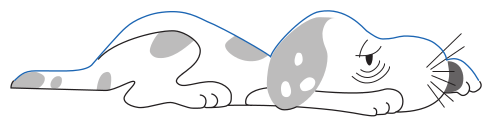
\includegraphics[width=0.6\textwidth]
		{puppy.png}
	\caption{The Noble Beast.}
\end{figure}
\begin{figure}
	\centering
	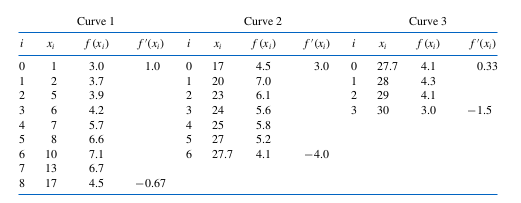
\includegraphics[width=0.8\textwidth]
		{data5.png}
	%\caption{Data - noble beast.}
\end{figure}

\newpage
\large \textbf{Answer 1.}
Dari penurunan dan algorithma yang diberikan di buku \textit{Numerical Analysis} oleh Richard L.Burden dan J. Douglas Faires, lalu dapat diterapkan untuk membuat program \textit{Cubic Spline Interpolation}. Setelah digabungkan \textit{Natural} dan \textit{Clamped Cubic Spline Interpolation} hasilnya sebagai berikut (\textit{spline.cpp}).

\begin{small}
\begin{verbatim}
/*****************************************************/
/* spline.cpp - Cubic Spline Interpolation           */
/* Natural and Clamped Spline                        */
/* Copyleft (c) 2012. Ridlo W. Wibowo                */
/*****************************************************/

#include <iostream>
#include <stdlib.h>
#include <math.h>
#include <fstream>
using namespace std;

double x[100], y[100]; // data - maksimal 100 data
//double A[100][100]; // Ac=alpha
double L[100], U[100], z[100], c[100], alpha[100], h[100];
double b[100], d[100]; // konstanta = y, b, c, d
int N=-1, n; // inisiasi jumlah data (N -> N = n+1)
double FPO, FPN;

void natural();
void clamped();
void plot();
double fx(double a, double b, double c, double d, double xi, double xh);
void spline_plot();
void fnatural();
void fclamped();

int main(){ 
    cout << "#### Cubic Spline Interpolation ####\n";

    // baca data
    ifstream read("data.txt");
    while (!read.eof()){
        N += 1;
        read >> x[N] >> y[N];
        //cout << x[N] << " " << y[N] << endl; 
    }
    read.close();
    cout << "Jumlah data : " << N << endl;
    n = N-1;
    //for (int i=0;i<n;i++){cout << x[i] << " " << y[i] << "\n";}
        
    // pilihan metode spline
    int ans;
    cout << "Choose the method: \n";
    cout << "1. Natural Cubic Spline\n";
    cout << "2. Clamped Cubic Spline\n";
    cout << "3. Both\n";
    cout << "Answer (1/2/3) : "; cin >> ans;
    if (ans == 1){fnatural();}
    else if (ans == 2){fclamped();}
    else if (ans == 3){fnatural(); fclamped();}
    else {cout << "Cancel program ... \n";}

    return 0;
}

void fnatural(){
    cout << "### Natural Cubic Spline\n";
    natural(); 
    spline_plot(); 
    cout << "Change spline-plot.txt ...\n";
    plot();
    cout << "Finish ...\n";
}

void fclamped(){
    cout << "### Clamped Cubic Spline\n";
    cout << "f'(x[0]) = "; cin >> FPO;
    cout << "f'(x[N]) = "; cin >> FPN;
    clamped(); 
    spline_plot();
    cout << "Change spline-plot.txt ...\n";
    plot();
    cout << "Finish ...\n";
}

void natural(){
    for (int i=0;i<n;i++){h[i] = x[i+1] - x[i];}
    for (int i=1;i<n;i++){
        alpha[i] = (3./h[i])*(y[i+1] - y[i]) - (3./h[i-1])*(y[i] - y[i-1]);}
    
    // Crout method
    L[0]=1.; U[0]=0.; z[0]=0.;
    for (int i=1;i<n;i++){
        L[i] = 2.*(x[i+1] - x[i-1]) - h[i-1]*U[i-1];
        U[i] = h[i]/L[i];
        z[i] = (alpha[i] - (h[i-1]*z[i-1]))/L[i];}
    
    L[n]=1.; z[n]=0.; c[n]=0.;
    for (int j=n-1;j>=0;j--){
        c[j] = z[j] - U[j]*c[j+1];
        b[j] = (y[j+1] - y[j])/h[j] - h[j]*(c[j+1] + 2.*c[j])/3.;
        d[j] = (c[j+1] - c[j])/(3.*h[j]);}
    
    // output file -> konstanta
    ofstream out("natural.txt");
    for (int i=0;i<n;i++){
        out << y[i] << " " << b[i] << " " << c[i] << " " << d[i] << endl;}
    out.close();
    // output file -> fungsi
    ofstream outf("natural-fungsi.txt");
    for (int i=0;i<n;i++){
        outf << "S"<<i<<"(x) = "<<y[i]<<" + "<<b[i]<<"*(x - "<<x[i]<<") + "<<c[i]<<"*(x - "<<x[i]<<")**2. + "<<d[i]<<"*(x - "<<x[i]<<")**3." << endl;}
    outf.close();
}

void clamped(){
    for (int i=0;i<n;i++){h[i] = x[i+1] - x[i];}
    
    alpha[0] = 3.*(y[1] - y[0])/h[0] - 3.*FPO;
    alpha[n] = 3.*FPN - 3.*(y[n] - y[n-1])/h[n-1];
    for (int i=1;i<n;i++){
        alpha[i] = (3./h[i])*(y[i+1] - y[i]) - (3./h[i-1])*(y[i] - y[i-1]);}
    
    // Crout method
    L[0]=2.*h[0]; U[0]=0.5; z[0]=alpha[0]/L[0];
    for (int i=1;i<n;i++){
        L[i] = 2.*(x[i+1] - x[i-1]) - h[i-1]*U[i-1];
        U[i] = h[i]/L[i];
        z[i] = (alpha[i] - (h[i-1]*z[i-1]))/L[i];}

    L[n]= h[n-1]*(2. - U[n-1]); 
    z[n]= (alpha[n] - h[n-1]*z[n-1])/L[n];
    c[n]= z[n];    
    for (int j=n-1;j>=0;j--){
        c[j] = z[j] - U[j]*c[j+1];
        b[j] = (y[j+1] - y[j])/h[j] - h[j]*(c[j+1] + 2.*c[j])/3.;
        d[j] = (c[j+1] - c[j])/(3.*h[j]);}
    
    // output file -> konstanta
    ofstream out("clamped.txt");
    for (int i=0;i<n;i++){
        out << y[i] << " " << b[i] << " " << c[i] << " " << d[i] << endl;}
    out.close();
    // output file -> fungsi
    ofstream outf("clamped-fungsi.txt");
    for (int i=0;i<n;i++){
        outf << "S"<<i<<"(x) = "<<y[i]<<" + "<<b[i]<<"*(x - "<<x[i]<<") + "<<c[i]<<"*(x - "<<x[i]<<")**2. + "<<d[i]<<"*(x - "<<x[i]<<")**3." << endl;}
    outf.close();
}

double fx(double a, double b, double c, double d, double xi, double xh){
    return a + b*(xi-xh) + c*(xi-xh)*(xi-xh) + d*(xi-xh)*(xi-xh)*(xi-xh);}

void spline_plot(){
    // nyebar titik sesuai fungsi selang (S(xj)) yang sesuai, untuk lihat hasil
    double xi=x[0];
    double xf=x[n];
    double yi=y[0];
    int jum = 500;
    double dx = (xf-xi)/jum;

    ofstream splineOut;
    splineOut.open("spline-plot.txt");
    splineOut << xi << " " << yi << endl;
    for (int i=0;i<jum;i++){
        xi = xi+dx;
        for (int j=0;j<n;j++){
            if (xi >= x[j] && xi < x[j+1]){
                yi = fx(y[j], b[j], c[j], d[j], xi, x[j]);
                splineOut << xi << " " << yi << endl;}}}
    splineOut.close();
}

void plot(){
    ofstream ploter("plot.in");
    ploter << "# gnuplot input file\n";
    //ploter << "set yrange [-6:4]\n";
    //ploter << "set xrange [0:14]\n";
    ploter << "plot \"data.txt\", \"spline-plot.txt\" w d lc 3 \n";
    ploter.close();
    
    system("gnuplot -persist < plot.in");
}
\end{verbatim}
\end{small} 

\newpage
Hasil program untuk masukan data sebagai berikut.
\begin{figure}
	\centering
	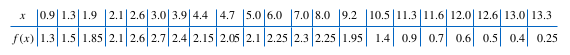
\includegraphics[width=0.85\textwidth]
		{data-burung.png}
	%\caption{Data - Burung.}
\end{figure}
\begin{figure}
	\centering
	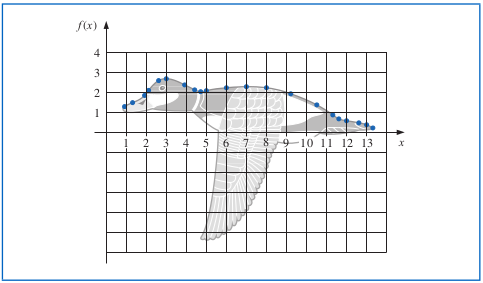
\includegraphics[width=0.7\textwidth]
		{burung.png}
	\caption{Plot - Burung.}
\end{figure}

\textit{Natural Spline}\\
dengan menggunakan program \textit{spline.cpp} di atas diperoleh:
\begin{figure}
	\centering
	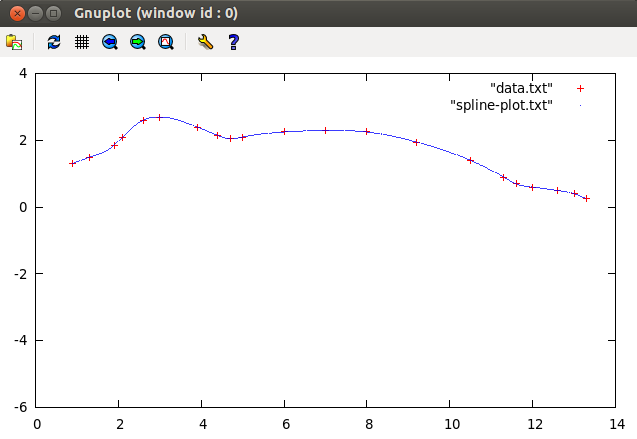
\includegraphics[width=0.65\textwidth]
		{natural-burung.png}
	\caption{\textit{Natural spline - program spline.cpp}.}
\end{figure}

\newpage
sebagai perbandingan, dengan menggunakan fungsi dari software \textit{gnuplot}:
\begin{verbatim} 
gnuplot > plot  ''data.txt'' smooth csplines 
\end{verbatim} 
diperoleh kurva yang sangat mirip sebagai berikut:
\begin{figure}
	\centering
	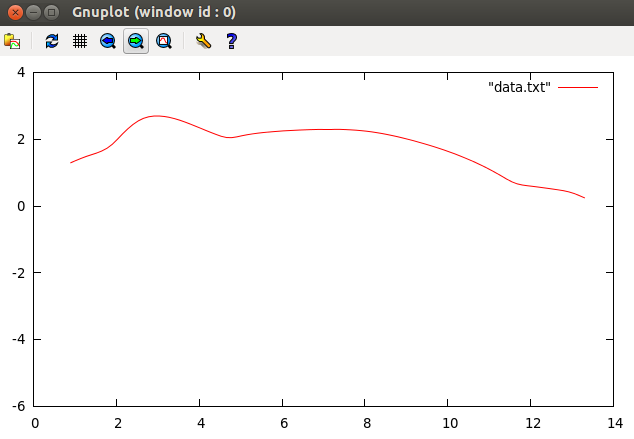
\includegraphics[width=0.65\textwidth]
		{gnuplot-burung-natural.png}
	\caption{\textit{Natural spline - gnuplot cubicspline}.}
\end{figure}

\textit{Clamped Spline}\\
dengan mengambil nilai sebarang misal: $f'(x[0]) = 3$ dan $f'(x[n]) = 3$, maka diperoleh hasil sebagai berikut.
\begin{figure}
	\centering
	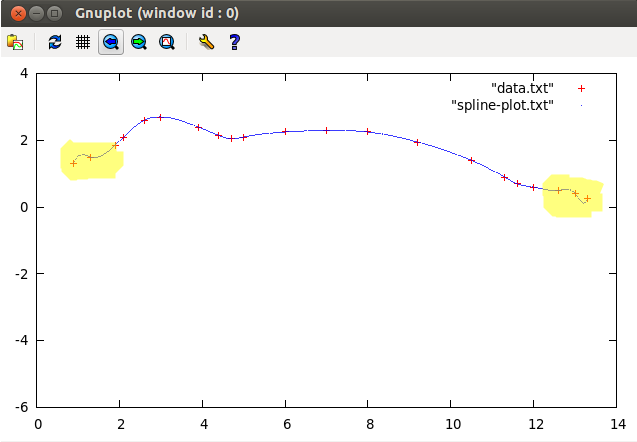
\includegraphics[width=0.7\textwidth]
		{clamped-burung.png}
	\caption{\textit{Clamped spline - spline.cpp}, terlihat perbedaan pada ujung kurva interpolasi karena menyesuaikan nilai input dari turunan di ujung.}
\end{figure}

\newpage
\large \textbf{Answer 2.} Menggunakan program \textit{spline.cpp} (natural spline) maka kita peroleh hasil sebagai berikut untuk tiap set data. \\ 
\textit{set data 1.} \\
konstanta,
\begin{small}
\begin{verbatim}
-0.6205 3.45509 0 -8.99579
-0.283987 3.18521 -2.69874 -0.946303
0.00660095 2.61708 -2.98263 9.9421
\end{verbatim}
\end{small}
atau fungsi tiap selang,
\begin{small}
\begin{verbatim}
S0(x) = -0.6205 + 3.45509*(x - 0.1) + 0*(x - 0.1)**2. + -8.99579*(x - 0.1)**3.
S1(x) = -0.283987 + 3.18521*(x - 0.2) + -2.69874*(x - 0.2)**2. + -0.946303*(x - 0.2)**3.
S2(x) = 0.00660095 + 2.61708*(x - 0.3) + -2.98263*(x - 0.3)**2. + 9.9421*(x - 0.3)**3.
\end{verbatim}
\end{small}
\begin{figure}
	\centering
	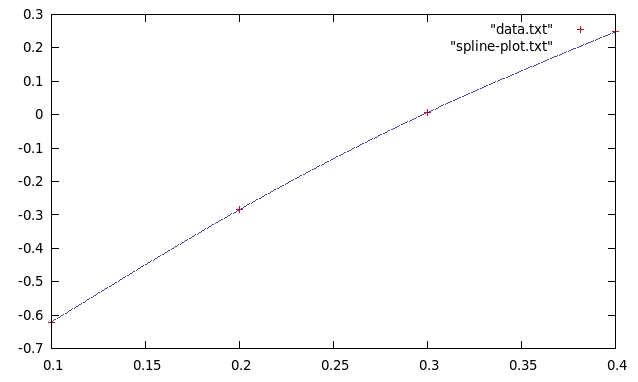
\includegraphics[width=0.45\textwidth]
		{spline-data1.png}
	\caption{\textit{Natural spline - set data 1}.}
\end{figure}

\textit{set data 2.}\\
konstanta,
\begin{small}
\begin{verbatim}
0.861995 0.175638 0 0.0656509
0.95802 0.224876 0.0984764 0.0282807
1.09861 0.344563 0.140897 -0.0939316
\end{verbatim}
\end{small}
atau fungsi tiap selang,
\begin{small}
\begin{verbatim}
S0(x) = 0.861995 + 0.175638*(x - -1) + 0*(x - -1)**2. + 0.0656509*(x - -1)**3.
S1(x) = 0.95802 + 0.224876*(x - -0.5) + 0.0984764*(x - -0.5)**2. + 0.0282807*(x - -0.5)**3.
S2(x) = 1.09861 + 0.344563*(x - 0) + 0.140897*(x - 0)**2. + -0.0939316*(x - 0)**3.
\end{verbatim}
\end{small}
\begin{figure}
	\centering
	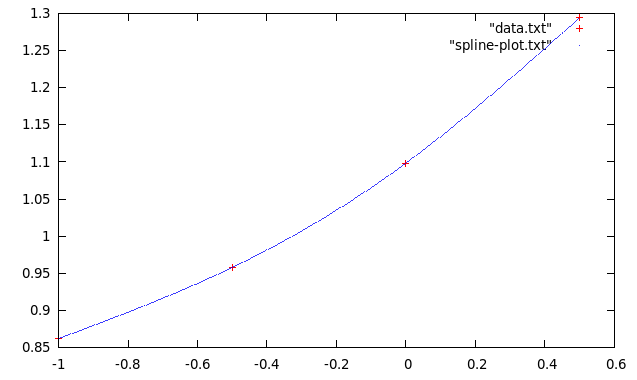
\includegraphics[width=0.45\textwidth]
		{spline-data2.png}
	\caption{\textit{Natural spline - set data 2}.}
\end{figure}

\large \textbf{Answer 3.} Nilai pendekatan dan errornya menggunakan fungsi dari interpolasi Spline.\\
\textit{\textbf{set data 1.}}\\
$f(x) = xcos(x) - 2x^{2} + 3x - 1$ \\
untuk $x = 0.25$ berada pada selang kedua, fungsi interpolasinya\\ 
$S1(x) = -0.283987 + 3.18521(x - 0.2) - 2.69874(x - 0.2)^{2} - 0.946303(x - 0.2)^{3}$\\
sehingga \\
$f(0.25) = -0.13277189457 $, \hspace{2cm} $S1(0.25) = -0.13159163787 $, \\
jadi $error = -0.0011802567$ \\ 

$f'(x) = -xsin(x)+cos(x)-4x+3$,\\
$S1'(x) = 3.18521 - 5.39748(x - 0.2) - 2.838909(x - 0.2)^{2} $, \\
$f'(0.25) = 2.9070614319 $, \hspace{2cm} $S1'(0.25) = 2.9082387275$, \\
jadi $error = -0.0011772956 $\\

\textit{\textbf{set data 2.}}\\
$f(x) = ln(e^{x} + 2)$ \\
untuk $x = 0.25$ berada pada selang ketiga, fungsi interpolasinya\\ 
$S2(x) = 1.09861 + 0.344563(x) + 0.140897(x)^{2} - 0.0939316(x)^{3}$\\
sehingga \\
$f(0.25) = 1.18906993111 $, \hspace{2cm} $S2(0.25) = 1.19208913125 $, \\
jadi $error = -0.0030192001$ \\ 

$f'(x) = \frac{e^{x}}{e^{x} + 2}$,\\
$S1'(x) = 0.344563 + 0.281794(x) - 0.2817948(x)^{2} $, \\
$f'(0.25) = 0.39099131515 $, \hspace{2cm} $S2'(0.25) = 0.397399325 $, \\
jadi $error = -0.006408009 $\\

\newpage
\large \textbf{Answer 4.} Menggunakan data yang ada pada soal dan program \textit{spline.cpp} (natural) menghasilkan interpolasi cubic spline sebagai berikut.\\

\textit{\textbf{Sample 1 average weight}}\\
konstanta,
\begin{small}
\begin{verbatim}
6.67 -0.44687 0 0.0617649
17.33 6.22374 1.11177 -0.270988
42.67 2.11045 -2.14009 0.281092
37.33 -3.14062 0.389736 -0.0141142
30.1 -0.700209 0.220366 -0.0249136
29.31 -0.0506808 -0.00385673 0.000160697
\end{verbatim}
\end{small}
atau fungsinya,
\begin{small}
\begin{verbatim}
S0(x) = 6.67 + -0.44687*(x - 0) + 0*(x - 0)**2. + 0.0617649*(x - 0)**3.
S1(x) = 17.33 + 6.22374*(x - 6) + 1.11177*(x - 6)**2. + -0.270988*(x - 6)**3.
S2(x) = 42.67 + 2.11045*(x - 10) + -2.14009*(x - 10)**2. + 0.281092*(x - 10)**3.
S3(x) = 37.33 + -3.14062*(x - 13) + 0.389736*(x - 13)**2. + -0.0141142*(x - 13)**3.
S4(x) = 30.1 + -0.700209*(x - 17) + 0.220366*(x - 17)**2. + -0.0249136*(x - 17)**3.
S5(x) = 29.31 + -0.0506808*(x - 20) + -0.00385673*(x - 20)**2. + 0.000160697*(x - 20)**3.
\end{verbatim}
\end{small}
plotnya, 
\begin{figure}
	\centering
	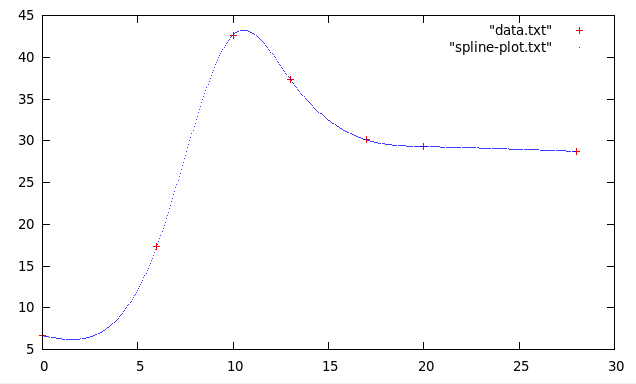
\includegraphics[width=0.8\textwidth]
		{sample1.png}
	\caption{\textit{Natural spline - Sample 1 average weight}.}
\end{figure}

\textit{\textbf{Sample 2 average weight}}\\
konstanta,
\begin{small}
\begin{verbatim}
6.67 1.66287 0 -0.00248723
16.11 1.39425 -0.0447702 -0.0325107
18.89 -0.524424 -0.434899 0.0591617
15 -1.53645 0.0975559 0.00226438
10.56 -0.647316 0.124729 -0.0111337
9.44 -0.199554 0.0245257 -0.0010219
\end{verbatim}
\end{small}
atau fungsinya,
\begin{small}
\begin{verbatim}
S0(x) = 6.67 + 1.66287*(x - 0) + 0*(x - 0)**2. + -0.00248723*(x - 0)**3.
S1(x) = 16.11 + 1.39425*(x - 6) + -0.0447702*(x - 6)**2. + -0.0325107*(x - 6)**3.
S2(x) = 18.89 + -0.524424*(x - 10) + -0.434899*(x - 10)**2. + 0.0591617*(x - 10)**3.
S3(x) = 15 + -1.53645*(x - 13) + 0.0975559*(x - 13)**2. + 0.00226438*(x - 13)**3.
S4(x) = 10.56 + -0.647316*(x - 17) + 0.124729*(x - 17)**2. + -0.0111337*(x - 17)**3.
S5(x) = 9.44 + -0.199554*(x - 20) + 0.0245257*(x - 20)**2. + -0.0010219*(x - 20)**3.
\end{verbatim}
\end{small}
plotnya, 
\begin{figure}
	\centering
	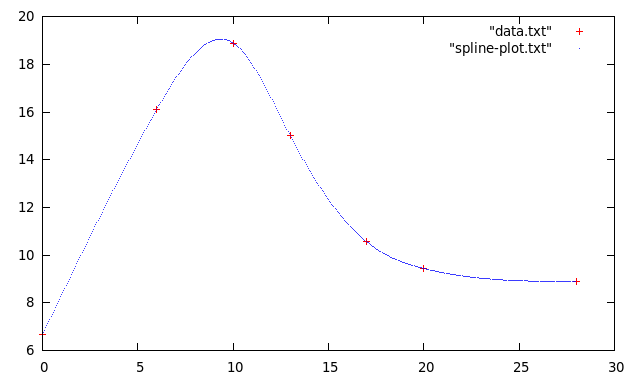
\includegraphics[width=0.8\textwidth]
		{sample2.png}
	\caption{\textit{Natural spline - Sample 2 average weight}.}
\end{figure}

Maksimum berat rata-rata untuk tiap sampel dapat diperoleh dari maksimum fungsi pada selang dimana maksimum interpolasi terjadi.\\

\textbf{Sampel 1} memiliki nilai maksimum pada selang ketiga ($S2(x)$), sehingga dapat dicari dengan menerapkan bahwa saat maksimum $S2'(x) = 0$.\\
\hspace{2cm} $S2(x) = 42.67 + 2.11045(x - 10) - 2.14009(x - 10)^{2} + 0.281092(x - 10)^{3}$\\
\hspace{2cm}$S2'(x) = 2.11045 - 4.28018(x - 10) + 0.843276(x - 10)^{2} = 0 $\\
dengan menggunakan rumus \textit{abc}, bisa kita peroleh solusi yang mungkin sesuai grafik di atas adalah pada saat $t_{max} = 10.55$ days dengan maksimum berat rata-rata $S2(t_{max}) = 43.23$ mg.\\

\textbf{Sampel 2} memiliki nilai maksimum pada selang kedua ($S1(x)$), dengan cara yang sama, kita peroleh hasil $t_{max} = 9.35$ days dengan maksimum berat rata-rata $S2(t_{max}) = 19.05$ mg.
%16.11 + 1.39425*(x - 6) + -0.0447702*(x - 6)**2. + -0.0325107*(x - 6)**3.
%1.39425 - 0.0895404*(x-6) - 0.0975321(x-6)^2.
%3.34964422254
%9.34964422254
%19.0560520195

\newpage
\large \textbf{Answer 5.}
Interpolasi dari bagian atas gambar ini dilakukan menggunakan metode \textit{Clamped Cubic Spline} menggunakan data yang ada pada soal. Menggunakan program \textit{spline.cpp} (clampled spline) dapat diperoleh interpolasi untuk 3 bagian kurva tersebut.\\
\begin{figure}
	\centering
	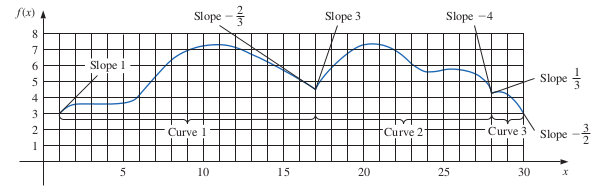
\includegraphics[width=1.0\textwidth]
		{puppy-ini.png}
	%\caption{Interpolasi.}
\end{figure}

hasil program \textit{spline.cpp} untuk 3 set data kurva beserta turunan di ujung-ujungnya apabila digabungkan menghasilkan plot sebagai berikut.
\begin{figure}
	\centering
	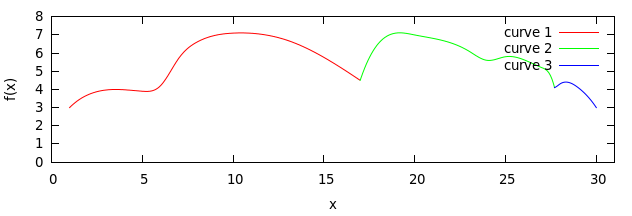
\includegraphics[width=1.0\textwidth]
		{curve321.png}
	\caption{Hasil program interpolasi - \textit{spline.cpp} (clamped).}
\end{figure}

dengan rincian fungsi tiap selang $S(x)$ sebagai berikut:\\

\textit{Curve 1}
\begin{small}
\begin{verbatim}
S0(x) = 3 + 1*(x - 1) + -0.34681*(x - 1)**2. + 0.04681*(x - 1)**3.
S1(x) = 3.7 + 0.44681*(x - 2) + -0.20638*(x - 2)**2. + 0.0265552*(x - 2)**3.
S2(x) = 3.9 + -0.0744797*(x - 5) + 0.0326168*(x - 5)**2. + 0.341863*(x - 5)**3.
S3(x) = 4.2 + 1.01634*(x - 6) + 1.05821*(x - 6)**2. + -0.574548*(x - 6)**3.
S4(x) = 5.7 + 1.40911*(x - 7) + -0.665439*(x - 7)**2. + 0.156329*(x - 7)**3.
S5(x) = 6.6 + 0.54722*(x - 8) + -0.19645*(x - 8)**2. + 0.0239201*(x - 8)**3.
S6(x) = 7.1 + 0.0484602*(x - 10) + -0.0529297*(x - 10)**2. + -0.00255607*(x - 10)**3.
S7(x) = 6.7 + -0.338131*(x - 13) + -0.0759343*(x - 13)**2. + 0.00574178*(x - 13)**3.
\end{verbatim}
\textit{Curve 2}
\end{small}
\begin{small}
\begin{verbatim}
S0(x) = 4.5 + 3*(x - 17) + -1.10071*(x - 17)**2. + 0.126162*(x - 17)**3.
S1(x) = 7 + -0.197875*(x - 20) + 0.0347502*(x - 20)**2. + -0.0229307*(x - 20)**3.
S2(x) = 6.1 + -0.608501*(x - 23) + -0.171626*(x - 23)**2. + 0.280127*(x - 23)**3.
S3(x) = 5.6 + -0.111371*(x - 24) + 0.668756*(x - 24)**2. + -0.357385*(x - 24)**3.
S4(x) = 5.8 + 0.153987*(x - 25) + -0.403398*(x - 25)**2. + 0.0882022*(x - 25)**3.
S5(x) = 5.2 + -0.401178*(x - 27) + 0.125815*(x - 27)**2. + -2.568*(x - 27)**3.
\end{verbatim}
\textit{Curve 3}
\end{small}
\begin{small}
\begin{verbatim}
S0(x) = 4.1 + 0.33*(x - 27.7) + 2.26205*(x - 27.7)**2. + -3.79941*(x - 27.7)**3.
S1(x) = 4.3 + 0.661386*(x - 28) + -1.15743*(x - 28)**2. + 0.29604*(x - 28)**3.
S2(x) = 4.1 + -0.765347*(x - 29) + -0.269307*(x - 29)**2. + -0.0653465*(x - 29)**3.
\end{verbatim}
\end{small}

\begin{figure}
	\centering
	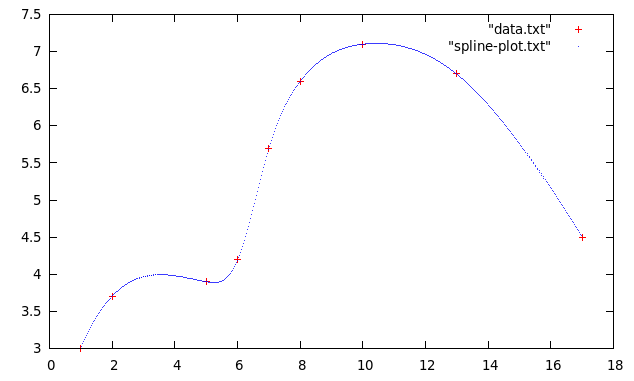
\includegraphics[width=0.4\textwidth]
		{curve1.png}
	\caption{Curve 1 - \textit{spline.cpp} (clamped).}
\end{figure}
\begin{figure}
	\centering
	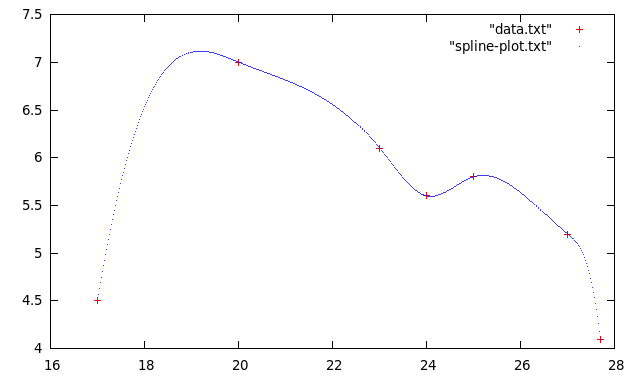
\includegraphics[width=0.4\textwidth]
		{curve2.png}
	\caption{Curve 2 - \textit{spline.cpp} (clamped).}
\end{figure}
\begin{figure}
	\centering
	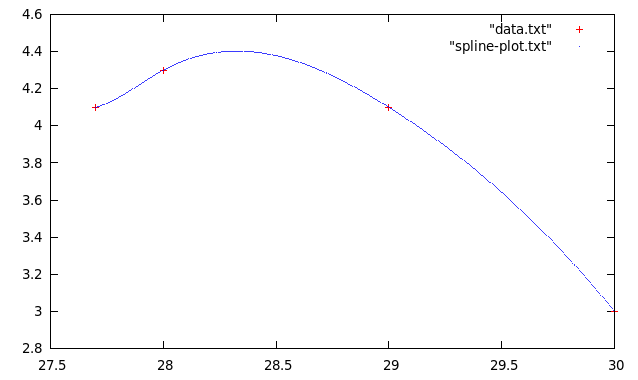
\includegraphics[width=0.4\textwidth]
		{curve3.png}
	\caption{Curve 3 - \textit{spline.cpp} (clamped).}
\end{figure}


\end{document}














